%% \documentclass[aspectratio=43]{beamer}
\documentclass[aspectratio=169]{beamer}
\usetheme[
  block=fill,
  background=light,
  titleformat=smallcaps,
  progressbar=frametitle,
  numbering=none,
]{metropolis}
\setbeamersize{text margin left=.7cm,text margin right=.7cm}
\usepackage{appendixnumberbeamer}

%%%%%%%%%%%%%%%%%%%%%%%%%%%%%%%%%%%%%%%%%%
%% Packages
%%%%%%%%%%%%%%%%%%%%%%%%%%%%%%%%%%%%%%%%%%

\usepackage[backend=bibtex,style=authoryear]{biblatex}

% Tikz
\usepackage{tikz}
\usetikzlibrary{arrows,positioning,matrix,fit,backgrounds,decorations.text,decorations.pathmorphing,calc,shapes}

% Colors
\usepackage{xcolor}
\usepackage{contour}

% Images
\usepackage{graphics}
\graphicspath{{img/}}

% Inference rules
\usepackage{amssymb}
\usepackage{stmaryrd}
\usepackage{proof}
\newenvironment{proposition}[1]
  {\begin{alertblock}{#1}\begin{displaymath}}
  {\end{displaymath}\end{alertblock}}

% Cross-out formulas
\usepackage[makeroom]{cancel}

% Colorboxes around formulas
\usepackage{fancybox}

%%%%%%%%%%%%%%%%%%%%%%%%%%%%%%%%%%%%%%%%%%
%% Macros
%%%%%%%%%%%%%%%%%%%%%%%%%%%%%%%%%%%%%%%%%%
\renewcommand\alert[1]{\textcolor{mLightBrown}{#1}}
\newcommand\todo[1]{\textcolor{red}{#1}}

%%%%%%%%%%%%%%%%%%%%%%%%%%%%%%%%%%%%%%%%%%
%% Fonts
%%%%%%%%%%%%%%%%%%%%%%%%%%%%%%%%%%%%%%%%%%
\usepackage{relsize}
\usepackage[tt=false]{libertine}
\usepackage[libertine]{newtxmath}

\usepackage{yfonts}
\usepackage{xspace}
\newcommand\I{\textgoth{I}\xspace}
\newcommand\II{\textgoth{II}\xspace}
\newcommand\III{\textgoth{III}\xspace}
\newcommand\IV{\textgoth{IV}\xspace}

\newcommand\agdatohs{\textsc{agda2hs}\xspace}

%----------------------------------------------------------------------------

\title{PhD Viva}
%\subtitle{}
\vspace{-2cm}
\author{Orestis Melkonian}
\date{December 8, 2023}
\titlegraphic{
\vspace*{6cm}

\includegraphics[keepaspectratio=true,height=1.2cm]{uoe}\hfill

\includegraphics[keepaspectratio=true,height=1.0cm]{iohk}
}

\begin{document}

\begin{center}
\setbeamerfont{title}{size=\large}
\setbeamerfont{subtitle}{size=\small}
\maketitle
\setbeamerfont{title}{size=\Large}
\setbeamerfont{subtitle}{size=\large}
\end{center}

\tikzset{
  % global
  every matrix/.style =
  { ampersand replacement = \&,
    matrix of nodes,
    nodes in empty cells },
  % nodes
  boxx/.style = {align = center},
  box/.style =
  { %draw, rectangle,
    align          = center,
    minimum width  = .5cm,
    minimum height = 1.5cm },
  BG/.style =
  { rectangle,
    inner sep       = 0.2cm,
    rounded corners = 5mm,
    line width      = 1mm },
  MSc/.style =
  { BG, fill=yellow!25, text=yellow!25 },
  MSc-label/.style =
  { label={[name=msc]above left:\contour{yellow!25}{}} },
  PhD/.style =
  { BG, fill=orange!20, text=orange!20 },
  PhD-label/.style =
  { label={[name=phd]below:\contour{orange!20}{}} },
  PhD2/.style =
  { BG, fill=orange!30, text=orange!30 },
  PhD2-label/.style =
  { label={[name=phd]#1:\contour{orange!30}{}} },
  PhD3/.style =
  { BG, fill=green!25, text=green!25 },
  PhD3-label/.style =
  { label={[name=phd]#1:\contour{green!25}{}} },
  greenBox/.style =
  { BG, fill=green!15, },
%%   greenDot/.style =
%%   { BG , left color = red!35, middle color = green!55
%%   , bottom color = green!55, right color = green!55 },
  redDot/.style =
  { BG, draw=red!55, dashed },
  %% font=\small,
  txt/.style    = {align=center},
  note/.style   = {font=\small\itshape},
  accept/.style = {fill = green!15},
  reject/.style = {fill = red!15},
  cit/.style =
  { inner sep = 0.3cm, rounded corners = 2mm, font=\normalsize, align=center },
  % edges
  to/.style = {->, thick},
  squig/.style = {decorate, decoration={zigzag}}
}

\newcommand\bitml{
  \matrix (mat)
    [ column sep = 1.5cm,
      row sep = 2cm,
      every node/.style = txt
    ] {
    \node {\textbf{\underline{Syntax}}};
    \& \node (operA) {};
    \& \node (operB) {};
    \& \node {\textbf{\underline{Game-theoretic}}\\\textbf{\underline{Semantics}}}; \\[-1cm]
    \node (contracts) {BitML\\Contracts};
    \& \node (lts) {Small-step\\LTS};
    \& \node (sm) {Symbolic\\Runs};
    \& \node (ss) {Symbolic\\Strategies}; \\
    \node (transactions) {Bitcoin\\Transactions};
    \& \node (bc) {Blockchain\\Consistency};
    \& \node (cm) {Computational\\Runs};
    \& \node (cs) {Computational\\Strategies}; \\
  };
  \node[fit=(operA)(operB)]{\textbf{\underline{Operational Semantics}}};
  \path
  (contracts) edge[to]
    node[right] (comp) {$\mathcal{C}$}
  (transactions)
  (sm) edge[<->, bend left = 40]
    node[right] (coh) {$\sim$}
  (cm)
  (cm) edge[to]
    node[left] (parsing) {\textit{\alert{parse}}}
  (sm)
  (ss) edge[to]
    node[left] (n) {$\aleph$}
  (cs)
  (coh.east) edge[<->, double]
    node[above] (compsA) {\textit{\alert{computational}}}
    node[below] (compsB) {\textit{\alert{soundness}}}
  (n.west)
  (lts) edge[squig] (sm)
  (bc) edge[squig] (cm)
  ;
}


\begin{frame}{BitML Progress}
\vspace{-1cm}
\begin{center}
\begin{tikzpicture}
\bitml
\begin{pgfonlayer}{background}
\node[MSc, MSc-label, fit=(contracts) (sm)] {};
\node[PhD, PhD-label, fit=(transactions) (cm)] {};
\node[PhD, fit=(contracts.south) (comp) (transactions)] {};
\node[PhD2, PhD2-label={above}, fit=(sm.east) (ss)] {};
\node[PhD2, PhD2-label={below}, fit=(cm.east) (cs)] {};
\node[redDot, fit=(sm.south east) (coh.east) (cm.north east)] {};
\end{pgfonlayer}
\end{tikzpicture}
\end{center}
\end{frame}

\begin{frame}{BitML paper: coherence relation}
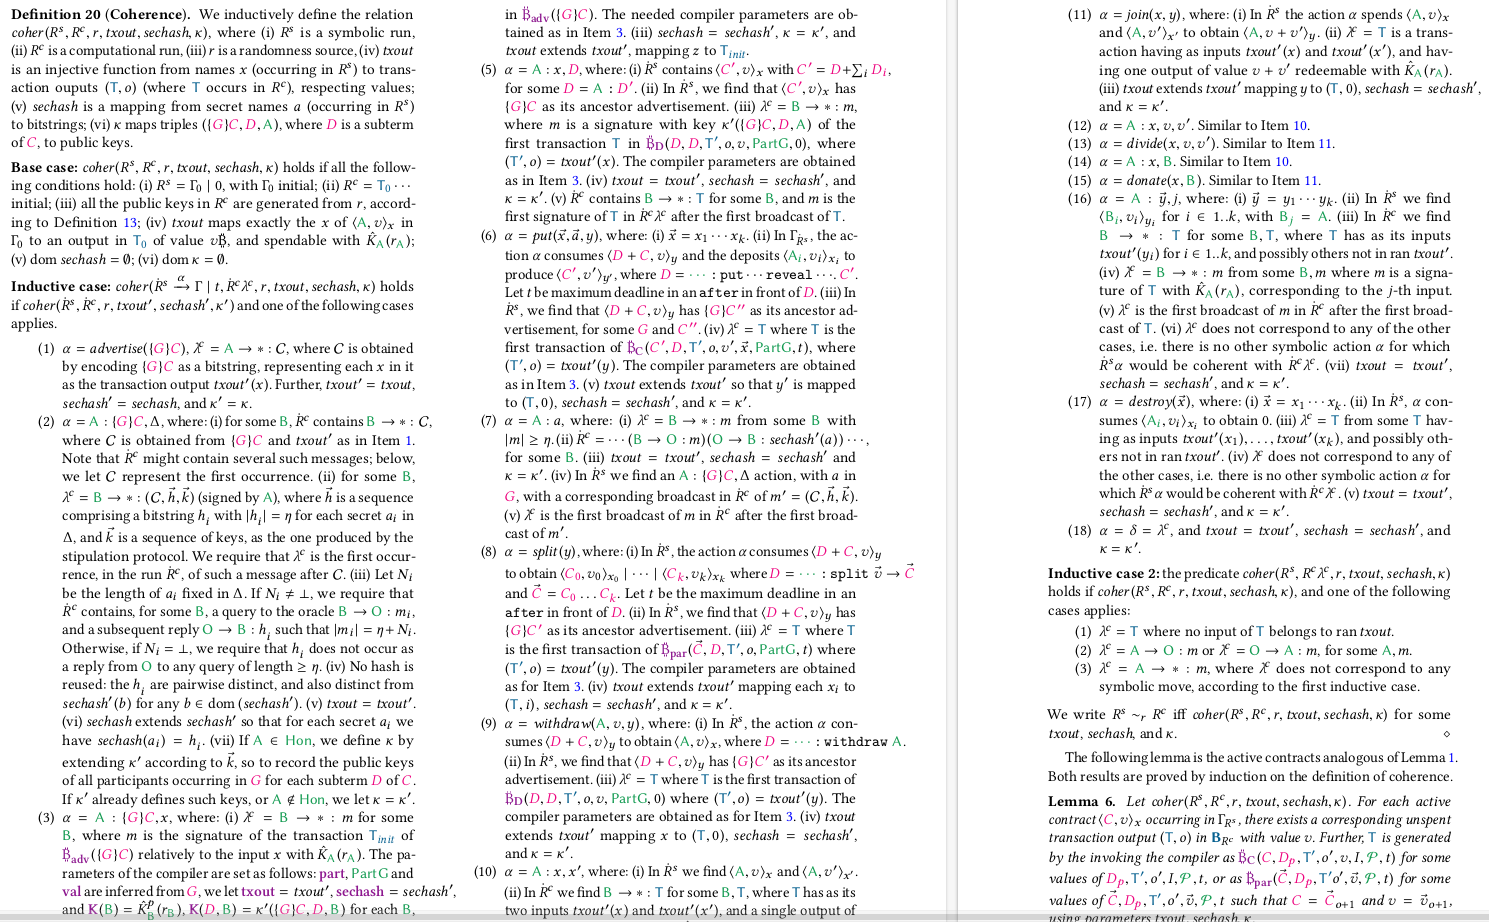
\includegraphics[keepaspectratio=true,height=\textheight]{bitml-coherence}
\end{frame}

\begin{frame}{Technical challenges for coherence}
\begin{itemize}
\item Proofs that construct mappings required \alert{meta-properties} on lists
\item Tracing a contract's lifetimer required \alert{temporal hyper-properties}
\item Scaling up $\to$ hit Agda's \alert{type-checking performance} limits
\end{itemize}
\end{frame}

\begin{frame}{BitML}
\vspace{-1cm}
\begin{center}
\begin{tikzpicture}
\bitml
\begin{pgfonlayer}{background}
\node[MSc, MSc-label, fit=(contracts) (sm)] {};
\node[PhD, PhD-label, fit=(transactions) (cm)] {};
\node[PhD, fit=(contracts.south) (comp) (transactions)] {};
\node[PhD2, PhD2-label={above}, fit=(sm.east) (ss)] {};
\node[PhD2, PhD2-label={below}, fit=(cm.east) (cs)] {};
\node[PhD3, PhD3-label={right, xshift=-1cm, yshift=.8cm}, fit=(sm.south east) (coh.east) (cm.north east)] {};
\node[redDot, fit=(parsing)] {};
\node[redDot, fit=(ss.south) (n) (cs.north)] {};
\end{pgfonlayer}
\end{tikzpicture}
\end{center}
\end{frame}

\begin{frame}{BitML paper: computational soundness}
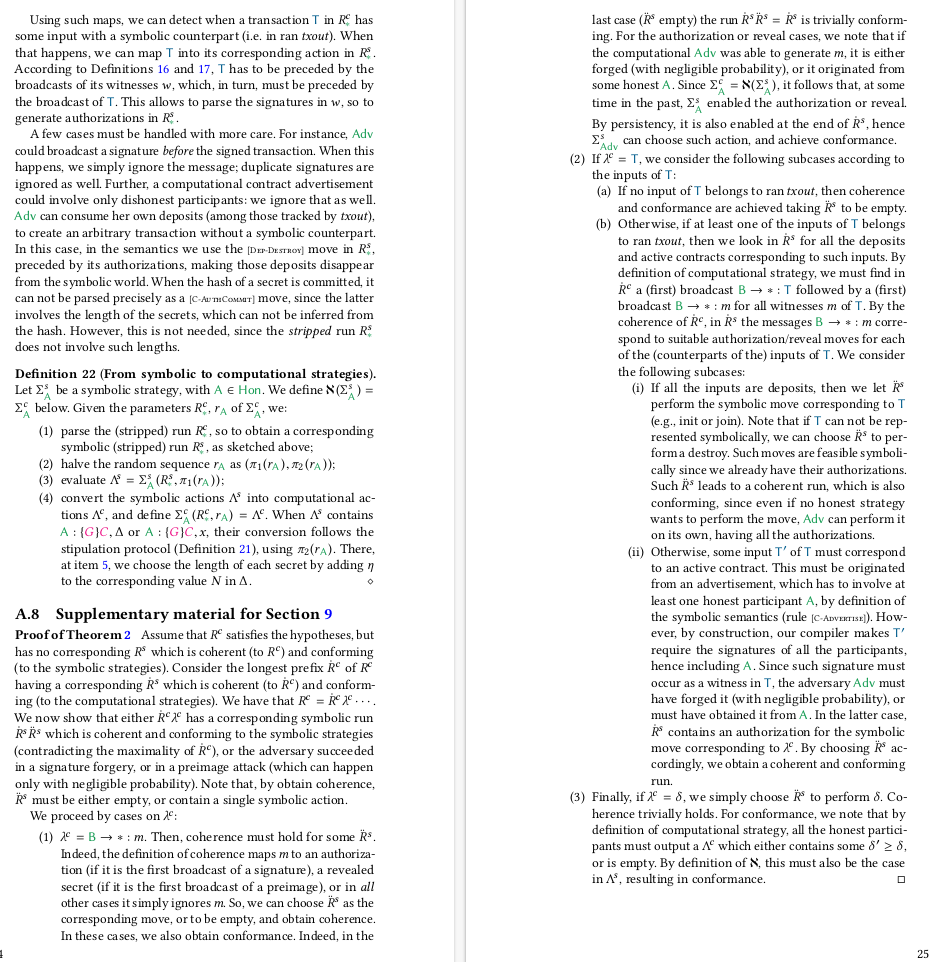
\includegraphics[keepaspectratio=true,height=\textheight]{bitml-theorem}
\end{frame}

\begin{frame}{BitML: Factoring out the non-game-theoretic part of the final theorem}

Given a computational run $R^c$ and symbolic strategies $\sigma^s$:

\[
\infer
  {\colorbox{green!20}{$\exists R^s. \ R^s \sim R^c$}
   \colorbox{red!20}{$\quad R^s$ conforms to $\Sigma^s$}}
  {\colorbox{green!20}{$R^c$} \colorbox{red!20}{conforms to $\Sigma^c \quad$
  where $\Sigma^c$ := $\aleph(\Sigma^s)$}}
\]

\begin{alertblock}{BACKUP PLAN}
Formalize only the first half of \textit{computational soundness} (i.e. \alert{parsing}).
\end{alertblock}
\end{frame}

\begin{frame}[standout]
\Large{επιστήμη}
\end{frame}

\end{document}
